\documentclass[tikz,border=4pt]{standalone}

\usepackage{amsmath,bm}
\usetikzlibrary{positioning,arrows.meta}

\tikzset{
  font=\sffamily,
  split/.style={draw, rounded corners, inner sep=.45em, fill=blue!15},
  leaf/.style={draw, rounded corners, inner sep=.45em},
  edgelbl/.style={font=\sffamily\scriptsize, inner sep=1pt},
}

\begin{document}
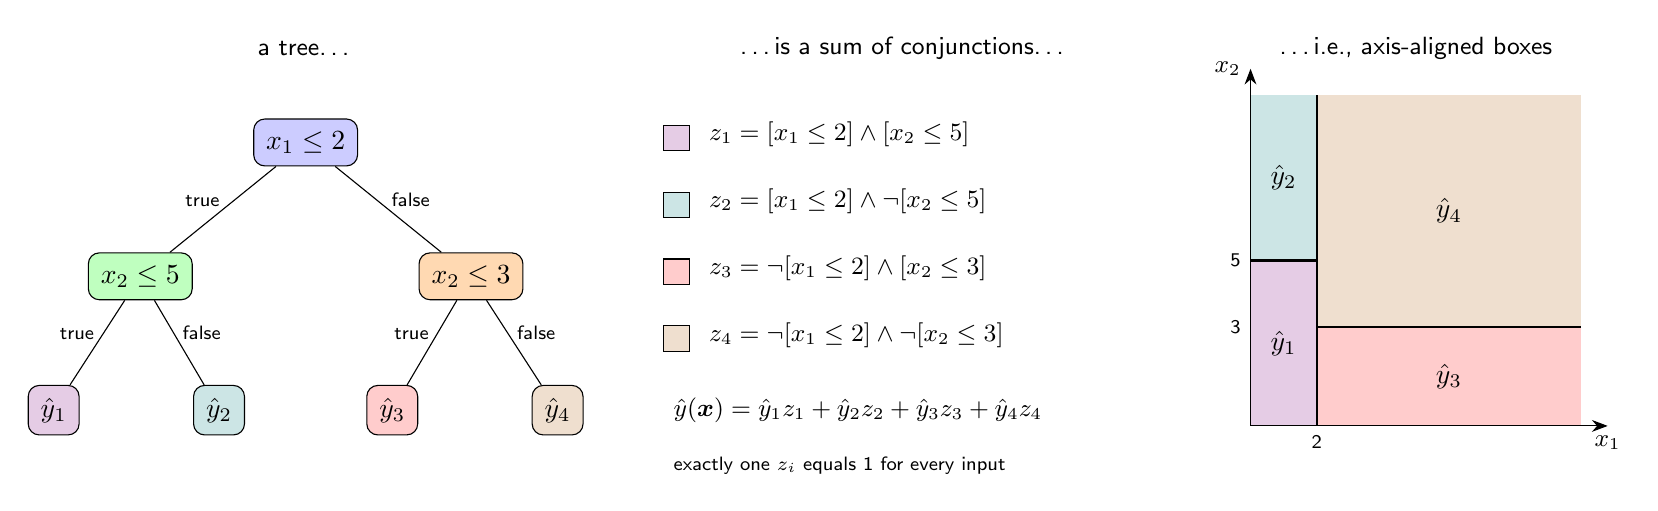
\begin{tikzpicture}[x=1cm, y=1cm]

  % ---------------- the decision tree ----------------
  \node[split, fill=blue!20]   (t1) at (0, 0)       {$x_1 \le 2$};
  \node[split, fill=green!25]  (t2) at (-2.1, -1.7) {$x_2 \le 5$};
  \node[split, fill=orange!30] (t3) at (2.1, -1.7)  {$x_2 \le 3$};
  \node[leaf, fill=violet!20] (l1) at (-3.2, -3.4) {$\hat y_1$};
  \node[leaf, fill=teal!20]   (l2) at (-1.1, -3.4) {$\hat y_2$};
  \node[leaf, fill=red!20]    (l3) at (1.1, -3.4)  {$\hat y_3$};
  \node[leaf, fill=brown!25]  (l4) at (3.2, -3.4)  {$\hat y_4$};

  \draw (t1) -- node[edgelbl, above left] {true} (t2);
  \draw (t1) -- node[edgelbl, above right] {false} (t3);
  \draw (t2) -- node[edgelbl, above left] {true} (l1);
  \draw (t2) -- node[edgelbl, above right] {false} (l2);
  \draw (t3) -- node[edgelbl, above left] {true} (l3);
  \draw (t3) -- node[edgelbl, above right] {false} (l4);

  % ---------------- the conjunctions ----------------
  \node[font=\sffamily\small, anchor=west] at (5.0, 0.1)  {$z_1 = [x_1 \le 2] \wedge [x_2 \le 5]$};
  \node[font=\sffamily\small, anchor=west] at (5.0, -0.75) {$z_2 = [x_1 \le 2] \wedge \neg[x_2 \le 5]$};
  \node[font=\sffamily\small, anchor=west] at (5.0, -1.6)  {$z_3 = \neg[x_1 \le 2] \wedge [x_2 \le 3]$};
  \node[font=\sffamily\small, anchor=west] at (5.0, -2.45) {$z_4 = \neg[x_1 \le 2] \wedge \neg[x_2 \le 3]$};
  \draw[fill=violet!20] (4.55, -0.1) rectangle ++(.32, .32);
  \draw[fill=teal!20]   (4.55, -0.95) rectangle ++(.32, .32);
  \draw[fill=red!20]    (4.55, -1.8) rectangle ++(.32, .32);
  \draw[fill=brown!25]  (4.55, -2.65) rectangle ++(.32, .32);
  \node[font=\sffamily\small, anchor=west] at (4.55, -3.4)
    {$\hat y(\bm x) = \hat y_1 z_1 + \hat y_2 z_2 + \hat y_3 z_3 + \hat y_4 z_4$};
  \node[font=\sffamily\scriptsize, anchor=west] at (4.55, -4.1)
    {exactly one $z_i$ equals 1 for every input};

  % ---------------- the induced partition ----------------
  \begin{scope}[shift={(12.0, -3.6)}, x=.42cm, y=.42cm]
    \fill[violet!20] (0, 0) rectangle (2, 5);
    \fill[teal!20]   (0, 5) rectangle (2, 10);
    \fill[red!20]    (2, 0) rectangle (10, 3);
    \fill[brown!25]  (2, 3) rectangle (10, 10);
    \draw[thick] (2, 0) -- (2, 10);
    \draw[thick] (0, 5) -- (2, 5);
    \draw[thick] (2, 3) -- (10, 3);
    \node at (1, 2.5)  {$\hat y_1$};
    \node at (1, 7.5)  {$\hat y_2$};
    \node at (6, 1.5)  {$\hat y_3$};
    \node at (6, 6.5)  {$\hat y_4$};
    \draw[-{Stealth[length=2mm]}] (0, 0) -- (10.8, 0) node[below, font=\sffamily\small] {$x_1$};
    \draw[-{Stealth[length=2mm]}] (0, 0) -- (0, 10.8) node[left, font=\sffamily\small] {$x_2$};
    \node[font=\sffamily\scriptsize, below] at (2, 0) {2};
    \node[font=\sffamily\scriptsize, left] at (0, 5) {5};
    \node[font=\sffamily\scriptsize, left] at (0, 3) {3};
  \end{scope}

  \node[font=\sffamily\small] at (0, 1.2) {a tree\dots};
  \node[font=\sffamily\small] at (7.6, 1.2) {\dots is a sum of conjunctions\dots};
  \node[font=\sffamily\small] at (14.1, 1.2) {\dots i.e., axis-aligned boxes};
\end{tikzpicture}
\end{document}
